
%% ==================================================================================================
%%
\documentclass[12pt]{book}
\usepackage{amsfonts}
\usepackage{amsmath}
\usepackage{amssymb}
\usepackage{graphicx}
\usepackage{hyperref}
\usepackage{float}
\usepackage{verbatim}
\usepackage{xlop} %% for multiplication https://tex.stackexchange.com/questions/11702/how-to-present-a-vertical-multiplication-addition
\usepackage{listings} %% to format generic computer code
\usepackage{lmodern} % for bold teletype font
\usepackage{minted} % colour Java code

\usepackage{tasks}
%\NewTasks[style=enumerate,counter-format=tsk[A].,label-width=3ex]{choice}[\item](4)

%% =======   set page margins    =======
\setlength{\textheight}{10in}
\setlength{\textwidth}{7.4in}
\setlength{\topmargin}{-0.75in}
\setlength{\oddsidemargin}{-0.5in}
\setlength{\evensidemargin}{-0.5in}
\setlength{\parskip}{0.15in}
\setlength{\parindent}{0in}

%%  for European long division
% https://tex.stackexchange.com/questions/432435/how-to-set-up-european-french-style-long-division-in-tex
\newcommand\frdiv[5]{%
    \[
    \renewcommand\arraystretch{1.5}
    \begin{array}{l| l}
    #1 & #2 \\
    \cline{2-2}
    #3 & #4 \\
    \cline{1-1}
    #5 & \\
    \end{array}
    \]
}

%%  for European long division


%% ==================================================================================================

\begin{document}

%\title{ITI1100 Digital Systems I}
%\author{Kien Do 300163370}
%\date{Assignment \#1}
\newcommand{\reporttitle}{Devoir 4}
\newcommand{\reportauthorOne}{Kien Do}
\newcommand{\cidOne}{300163370}
\input{titlePage/titlepage.txt}



%% ==================================================================================================

%%%%%%%%%%%% PROBLEMS START HERE

\begin{enumerate}
    \item \textbf{Réponse}

Python
\begin{minted}[breaklines,frame=single]{python}
# Puisque Python n'a pas introduit d'instructions à sélection multiple (match/case) avant Python 3.10 en 2021, j'utiliserai des instructions if/elif régulières pour cette partie du devoir.

if k == 1 or k == 2:
    j = 2 * k - 1
elif k == 3 or k == 5:
    j = 3 * k + 1
elif k == 4:
    j = 4 * k - 1
elif k == 6 or k == 7 or k == 8:
    j = k - 2
\end{minted}
Java
\begin{minted}[breaklines,frame=single]{java}
// Méthode "fall-through"
public class Main
{
    public static void main(String[] args) {
        int k = 1;
	int j = 0;
	
	switch(k) {
	    case 1:
	    case 2:
                j = 2 * k - 1;
                break;
            case 3:
	    case 5:
                j = 3 * k + 1;
                break;
            case 4:
                j = 4 * k - 1;
                break;
            case 6:
            case 7:
            case 8:
                j = k - 2;
                break;
        }
    }
}
\end{minted}
L'utilisation de plusieurs instructions à sélection multiple au lieu d'instructions conditionnelles if/else régulières augmente donc la fiabilité du programme.

% ===================================================================
\newpage
    \item \textbf{Réponse}\\
    
Segment de programme C sans \textbf{gotos} ni \textbf{breaks}.
\begin{minted}[breaklines,frame=single]{c}
#include <stdio.h>

int main()
{
    int j = -3;
    
    for (int i = 0; i < 3; i++) 
    {
        if ((j + 2) == 3 || (j + 2) == 2) 
        {
            j--;
        }
        else if ((j + 2) == 0) 
        {
            j += 2;
        }
        else
        {
            j = 0;
        }
        
        if (j > 0)
        {
            j = 3 - i;
        }
    }
   
    return 0;
}

\end{minted}

% ===================================================================
\newpage
    \item Affichez la pile avec toutes les instances d'enregistrement d'activation, y compris les chaînes statiques et dynamiques, lorsque l'exécution atteint la position 1 dans le programme squelette suivant. Supposons que bigsub est au niveau 1. (10pts)\\
    
    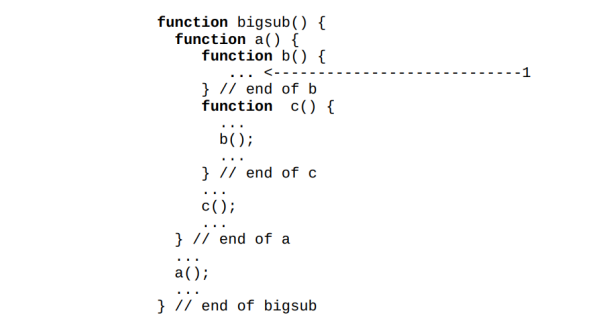
\includegraphics[scale=1]{D4_Q3_question.png}


\textbf{Réponse:}\\

    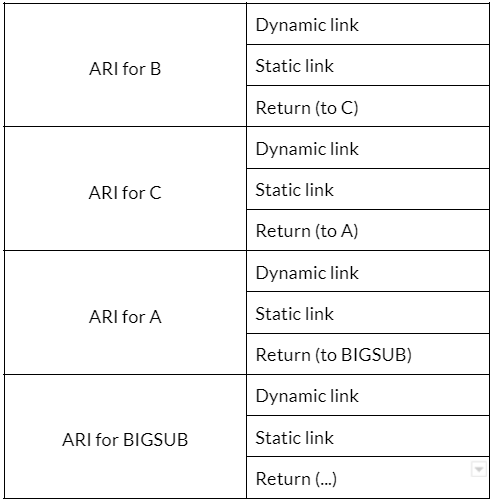
\includegraphics[scale=1]{D4_Q3_answer.png}

% ===================================================================
\newpage
    \item Affichez la pile avec toutes les instances d'enregistrement d'activation, y compris les chaînes statiques et dynamiques, lorsque l'exécution atteint la position 1 dans le programme squelette suivant. Supposons que bigsub est au niveau 1. (10pts)
    
    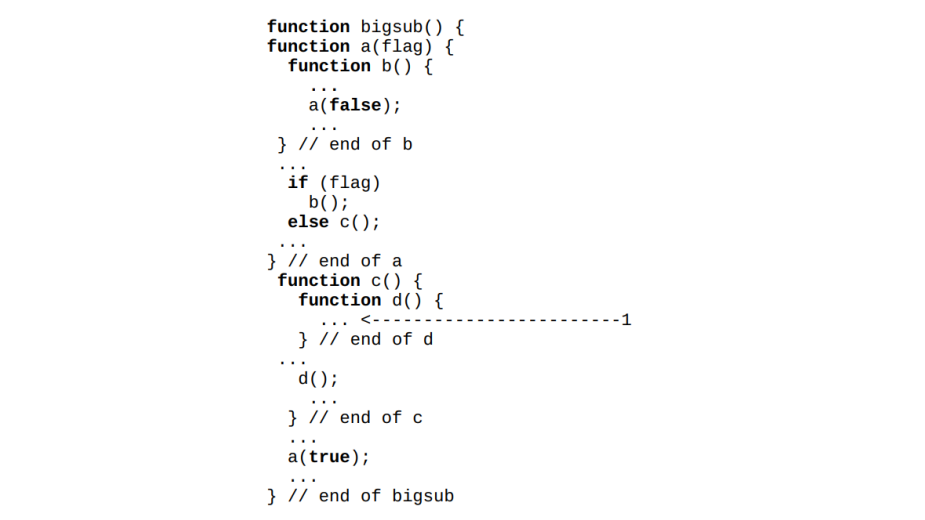
\includegraphics[scale=1]{D4_Q4_question.png} % 0.65

    La séquence d'appel de ce programme à exécuter pour atteindre $d$ est :\\
    --- bigsub appelle $a$.\\
    --- $a$ appelle $b$.\\
    --- $b$ appelle $a$.\\
    --- $a$ appelle $c$.\\
    --- $c$ appelle $d$.
    \\\\\\\\
    \underline{Remarque:} La réponse est sur la page suivante.

    \newpage
    
    \textbf{Réponse:}

    % 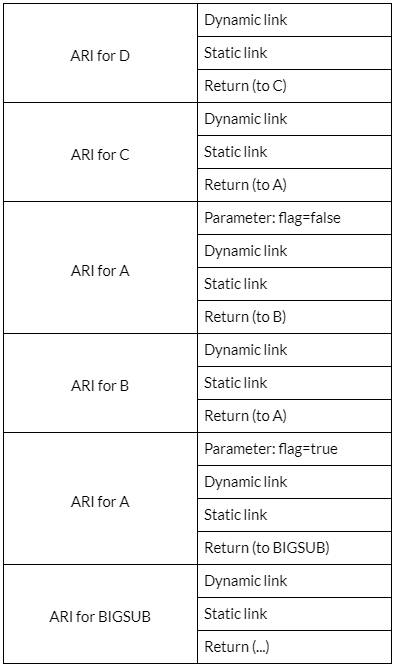
\includegraphics[scale=0.8]{D4_Q4_answer.png}
    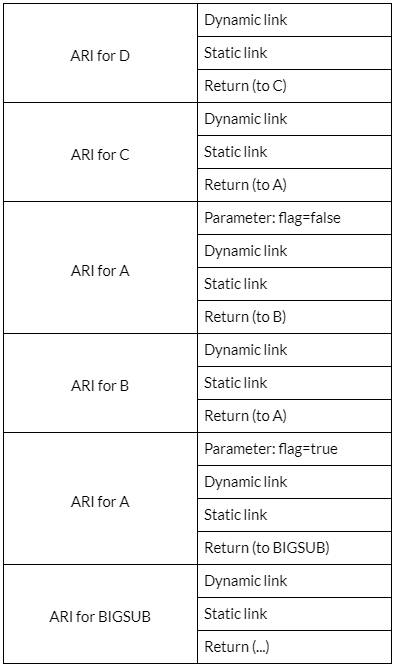
\includegraphics[scale=1.4]{D4_Q4_answer.png}





\end{enumerate}

\end{document} 
